% Exemplo de relatório técnico do IC
% Criado por P.J.de Rezende antes do Alvorecer da História.
% Modificado em 97-06-15 e 01-02-26 por J.Stolfi.
% Last edited on 2003-06-07 21:12:18 by stolfi

% modificado em 1o. de outubro de 2008

\documentclass[11pt,twoside]{article}
\usepackage{techrep-ic}
\usepackage[pdftex]{graphicx}
\usepackage{enumerate}

%%% SE USAR INGLÊS, TROQUE AS ATIVAÇÕES DOS DOIS COMANDOS A SEGUIR:
\usepackage[brazil]{babel}
%% \usepackage[english]{babel}

%%% SE USAR CODIFICAÇÃO LATIN1, TROQUE AS ATIVAÇÕES DOS DOIS COMANDOS A
%%% SEGUIR:
%% \usepackage[latin1]{inputenc}
\usepackage[utf8]{inputenc}

\begin{document}

%%% PÁGINA DE CAPA %%%%%%%%%%%%%%%%%%%%%%%%%%%%%%%%%%%%%%%%%%%%%%%
%
% Número do relatório
\TRNumber{45}

% DATA DE PUBLICAÇÃO (PARA A CAPA)
%
\TRYear{10} % Dois dígitos apenas
\TRMonth{05} % Numérico, 01-12

% LISTA DE AUTORES PARA CAPA (sem afiliações).
\TRAuthor{Birocchi, Anderson - RA: 072787 \and Braga, Felipe - RA:070803}

% TÍTULO PARA A CAPA (use \\ para forçar quebras de linha).
\TRTitle{MC823 - Laboratório de Redes\\Projeto 2: Servidor UDP Iterativo para Consulta a Banco de Dados de um Cinema}

\TRMakeCover

%%%%%%%%%%%%%%%%%%%%%%%%%%%%%%%%%%%%%%%%%%%%%%%%%%%%%%%%%%%%%%%%%%%%%%
% O que segue é apenas uma sugestão - sinta-se à vontade para
% usar seu formato predileto, desde que as margens tenham pelo
% menos 25mm nos quatro lados, e o tamanho do fonte seja pelo menos
% 11pt. Certifique-se também de que o título e lista de autores
% estão reproduzidos na íntegra na página 1, a primeira depois da
% página de capa.
%%%%%%%%%%%%%%%%%%%%%%%%%%%%%%%%%%%%%%%%%%%%%%%%%%%%%%%%%%%%%%%%%%%%%%

%%%%%%%%%%%%%%%%%%%%%%%%%%%%%%%%%%%%%%%%%%%%%%%%%%%%%%%%%%%%%%%%%%%%%%
% Nomes de autores ABREVIADOS e titulo ABREVIADO,
% para cabeçalhos em cada página.
%
\markboth{Birocchi, Braga}{MC823 - Projeto 2, Aplicação UDP}
\pagestyle{myheadings}

%%%%%%%%%%%%%%%%%%%%%%%%%%%%%%%%%%%%%%%%%%%%%%%%%%%%%%%%%%%%%%%%%%%%%%
% TÍTULO e NOMES DOS AUTORES, completos, para a página 1.
% Use "\\" para quebrar linhas, "\and" para separar autores.
%
\title{MC823 - Projeto 2, Servidor UDP Iterativo para Consulta a Banco de Dados de um Cinema}

\author{Anderson Birocchi, Felipe Braga}

\date{}

\newpage
\tableofcontents
\newpage

\maketitle

%%%%%%%%%%%%%%%%%%%%%%%%%%%%%%%%%%%%%%%%%%%%%%%%%%%%%%%%%%%%%%%%%%%%%%

\newenvironment{codelisting}
{\begin{list}{}{
\setlength{\leftmargin}{1em}
}
\item\scriptsize\bfseries}{\end{list}}


\begin{abstract}
Complementarmente ao anterior, o objetivo deste projeto é dar uma noção dos aspectos da implementação de um sistema que utiliza comunicação em rede. Desta vez, no entanto, foi usado o protocolo da camada de transporte UDP - \textit{User Datagram Protocol}. Procurou-se verificar as brechas geradas pela inconfiabilidade na entrega deste protocolo, assim como comparar a aplicação com a anterior, em TCP (tanto com relação à implementação como ao desempenho).
\end{abstract}

\section{Introdução}

Vimos no projeto anterior que os sockets TCP são ótimos para atividades que requerem robustez e segurança, como transações bancárias, armazenamento remoto de dados, transferência de arquivos em geral, etc. Porém, em troca dessa robustez e segurança, a velocidade da transmissão é prejudicada, já que no protocolo TCP há controle de fluxo, controle de congestionamento da rede e tratamento de perda de pacotes. Isso não costuma ser um problemas para as atividades citadas anteriormente, pois a velocidade não é algo crucial, no entanto, e se a atividade for uma transmissão ao vivo pela internet? A velocidade é fundamental, e a perda de alguns pacotes não condenam totalmente a transmissão.\\
Para esse e muitos outros casos, são utilizados sockets UDP, com comunicação sem conexão, apenas através de datagramas, que por não ter nenhum tipo de controle de fluxo, congestionamento ou perda de pacotes, consegue uma transmissão rápida porém não confiável de datagramas.\\
E se utilizarmos sockets UDP para o servidor de banco de dados de um cinema já implementado anteriormente? Será que a velocidade de comunicação realmente vai aumentar? Será que a perda de pacotes vai inviabilizar o uso da aplicação?\\
Nosso projeto irá reimplementar o servidor para consultas em bancos de dados de um cinema, mas agora utilizando sockets UDP na comunicação entre o servidor e o cliente.\\
A seção 2 irá especificar novamente o que exatamente o programa deve fazer; a seção 3 irá comentar mais detalhadamente a implementação, as definições, suposições tomadas e ferramentas utilizadas; a seção 4 irá analisar o desempenho da aplicação atraveś de várias medidas de tempo e também uma comparação dos tempos se utilizando TCP e UDP; a seção 5 irá mostrar quão não-confiável inconsistente é a aplicação se utilizando UDP; na seção 6 encontra-se uma breve conclusão sobre o projeto e, por último, na seção 6 estará o código fonte necessário para compilar e executar o servidor e o cliente.


\section{Casos de Uso}

Relembrando o que a aplicação deve fazer, segue abaixo uma listagem de 6 ações que serão implementadas. Nota: as ações com (*) precisam receber um identificador numérico do filme como entrada.\\
As ações sempre serão tomadas pelo cliente, sendo o servidor apenas quem irá processar o pedido. O resultado da ação apenas é vista pelo cliente que a iniciou, deixando o servidor totalmente à parte do que está acontecendo do lado dos seus clientes.
\subsection{Listar todas as informações de todos os filmes}
Mostrar o ID, título, sinopse, horário das sessões e as salas de todos os filmes cadastrados no banco de dados do servidor.
\subsection{Listar ID e título de todos os filmes}
Fazer uma busca rápida de todos os títulos e seus IDs, mais utilizado para auxiliar em futuras consultas, e utilização dos próximos casos de uso.
\subsection{Listar todas as informações de um filme (*)}
Buscar todas as informações sobre o filme com o dado ID.
\subsection{Mostrar a sinopse de um filme (*)}
Mostrar a sinopse completa do filme com o dado ID.
\subsection{Mostrar a avaliação de um filme (*)}
Mostrar a quantidade de votos o filme teve e qual foi a pontuação obtida.
\subsection{Avaliar um filme (*)}
Dar uma pontuação ao filme com o dado ID.



\section{Implementação}
Assim como no projeto anterior, o programa é desenvolvido na linguagem C e utiliza as bibliotecas padrão de comunicação do Unix. Desta vez, porém, são setadas as informações para o uso do UDP (\textit{DATAGRAM\_SOCKET}).\\
O funcionamento básico do sistema é: o cliente envia uma requisição ao servidor, que realiza alguma tarefa (caso necessário) e envia uma resposta ao cliente. Adiantamos que, diferentemente do TCP, a requisição é única, já contendo todas as informações que o servidor possa precisar.\\
No fim, a quantidade de linhas de código de todos os arquivos do sistema (*.c e *.h) é 1246 (aproximadamente 200 linhas a menos que com o TCP - essa diferença se deve às simplicidades geradas pela falta de complexidade do UDP, como será explicado posteriormente).\\
A seguir, serão pontuadas características do desenvolvimento em alguns assuntos que encontramos.\\

\subsection{Dados}
A forma como o sistema armazena os dados, tanto na camada de persistência (arquivo) como na de manipulação (memória) é exatamente a mesma que no primeiro projeto, de modo que o código necessário para a definição e manipulação dos dados foi reutilizado.\\
No entanto, é importante ressaltar que nem tudo que implementamos para o projeto usando TCP foi usado. A explicação disso é que, por causa do caráter de fluxo (\textit{streamming}) do TCP, e para minimizar disperdícios, as mensagens eram sempre enviadas como sequencias de caracteres, e era utilizado um caractere para sinalizar o fim da string. No caso do UDP, a comunicação é baseada em datagramas, e para cada registro que é enviado, um bloco de tamanho fixo é utilizado para comportar os dados do filme. Assim, apesar do desperdício de memória e de bytes sendo enviados pela rede, esta parte da implementação ficou consideravelmente mais simples, pela ausência da necessidade de tratamento do fim do fluxo.\\

\subsection{Protocolo de comunicação usando UDP}
Como o UDP não garante que os dados enviados serão recebidos, e se recebidos, podem chegar fora de ordem, foram implementada duas principais medidas para reger a comunicação:
\subsubsection{Do cliente para o servidor}
Anteriormente, com o uso do TCP, o cliente selecionava a opção, que era enviada ao servidor. No caso de se tratar de uma opção que requer um id, o cliente então lê e envia este id, enquanto no lado servidor a thread responsável por aquela conexão espera este id. O mesmo acontecia para a opção 6, que requer uma nota para avaliar o filme.\\
Como não há uma conexão de fato, seria pouco seguro continuar usando esta abordagem, uma vez que um cliente C1 poderia enviar uma opção que requer um id; e quando o servidor passasse a esperar pelo id, outro cliente C2 poderia enviar uma opção (que seria lida como id), e o programa ficaria inconsistente.\\
É possível pensar na comunicação do cliente com o servidor como uma pergunta e resposta, onde o cliente envia uma pergunta "atômica" (apenas um datagrama), de modo que o servidor sabe exatamente o que o cliente quer com apenas uma mensagem.\\
Para isso, foram empacotadas as informações: \textit{opção}, \textit{id} e \textit{nota} num vetor chamado \textit{request}, mesmo para as opções que não requerem id e/ou nota. O envio deste vetor é, então, a considerada pergunta "atômica" e suficiente.
\subsubsection{Do servidor para o cliente}
Depois de enviar uma pergunta ao servidor, o cliente passa a esperar pela resposta. Mas e se a resposta começar a demorar? O UDP não garante que as mensagens enviadas serão recebidas. Logo, tanto a pergunta como a resposta podem se perder. Assim, no caso de um ou outro, o cliente ficaria bloqueado infinitamente no \textit{recv()}, o que não é interessante.\\
Para contornar isso, implementamos um \textit{time-out} para o recebimento de respostas pelo cliente. Seu funcionamento se dá como segue:\\
\textbf{Ideia 1}\\
Toda vez que o cliente for receber uma resposta do servidor, entra num laço \textit{for()}, razoavelmente grande (por exemplo, de 1000 vezes). A cada iteração, é chamado o \textit{recv()} no modo não-bloqueante (a partir da configuração pela flag). Caso esse \textit{recv()} leia a resposta, sai do laço e sabe-se que nenhuma msg se perdeu. Caso contrário, é chamada uma função de espera \textit{sleep()}, de algum tempo curto (p.e, 100 micro-segundos) e terminado isso, volta ao início do laço. Caso o laço se encerre, sabe-se que a resposta não chegou até o \textit{time-out} e provavelmente ou a pergunta ou a resposta se perdeu.\\
No entanto, ao tentarmos efetuar a implementação, surgiram alguns problemas para conseguir fazer com o que o \textit{recv()} ficasse efetivamente não bloqueante. Tentou-se mudar todo o socket do cliente para não bloqueante, com a função \textit{fcntl()}, que também se mostrou ineficiente. Somado ao fato de este ser um método que faz o processo cliente ficar em espera ocupada (consumindo recursos do processador), optamos por implementar usando a função \textit{select()}.
\textbf{Ideia 2}\\
Dando uma grande facilidade, a função \textit{select()} implementa tanto um "ouvinte" para o socket de leitura, retornando quando algum datagrama chegou até ele, como o \textit{time-out}, tornando a codificação bem mais simples.\\

\subsection{Servidor iterativo X Servidor concorrente}
Em uma aplicação UDP não faz sentido se falar de múltiplas conexões, de concorrência ou de exclusão mútua, pois primeiro, não há conexão, o servidor é iterativo, ou seja, ao chegar um datagrama ele processa e responde ao cliente que pediu, e caso datagramas de outros clientes cheguem no socket UDP, estes ficam numa fila esperando o socket ficar livre novamente; e segundo, por ser iterativo, o servidor não vai permitir que dois ou mais clientes acessem ao mesmo tempo o banco de dados, evitando assim, concorrência e a necessidade de se garantir exclusão mútua.\\


\section{Análise de Tempo}
Para a análise de tempo, foi considerada apenas uma operação a ser analisada,o tempo de consulta ao servidor, já que o tempo de conexão (RTT) não faz mais sentido exatamente por não haver mais conexão.\\
Para se obter uma boa precisão, foi utilizada a função "gettimeofday", que tem a precisão em microsegundos, o que já é boa o suficiente para nossa aplicação. A função pega o tempo atual em que foi chamada, portanto, para calcular o tempo de alguma operação, basta calcular o tempo antes e depois da operação e calcular a diferença entre eles.\\
Foram usadas duas configurações:\\
\textbf{Configuração 1: }Dois computadores presentes na mesma sub-rede (SIFEEC).\\
IP local: 143.106.150.77\\
IP remoto: 143.106.150.74\\
\textbf{Configuração 2: }Um computador no laboratório do IC3 e outro no SIFEEC.\\
IP local: 143.106.150.77\\
IP remoto: 143.106.16.163 (xaveco)\\
\begin{verbatim}
[ra072787@xaveco ~]$ traceroute 143.106.150.74
traceroute to 143.106.150.74 (143.106.150.74), 30 hops max, 60 byte packets
 1  routeric3.lab.ic.unicamp.br (143.106.16.148)  2.801 ms  5.398 ms  7.873 ms
 2  143.106.16.150 (143.106.16.150)  0.099 ms  0.074 ms  0.065 ms
 3  143.106.7.129 (143.106.7.129)  0.218 ms  0.182 ms  0.159 ms
 4  area3-gw.unicamp.br (143.106.1.129)  0.570 ms  0.748 ms  0.981 ms
 5  ptp-nct-nbs.unicamp.br (143.106.199.13)  0.636 ms  0.870 ms  1.036 ms
 6  fee-gw.unicamp.br (143.106.1.10)  1.049 ms  1.332 ms  1.305 ms
 7  le20-10.grad.fee.unicamp.br (143.106.150.74)  2.070 ms  2.047 ms  2.401 ms
[ra072787@xaveco ~]$
\end{verbatim}
\textit{Observação: }Todos os tempos que serão mostrados nas próximas seções estão em micro-segundos, e pode-se verificar todos os valores encontrados na seção de Anexos.\\

\subsection{Tempo de Consulta}
Tempo decorrido entre o cliente realizar o caso de uso 1 (consulta completa de todos os filmes do banco de dados).\\
\textbf{Configuração 1: }\\
Média do tempo de consulta: \textbf{2288,52 us}\\
Desvio padrão: \textbf{792,62 us}\\
\textbf{Configuração 2: }\\
Média do tempo de consulta: \textbf{3606,54 us}\\
Desvio padrão: \textbf{1094,37 us}\\
\begin{figure}[htb]
  \centering
  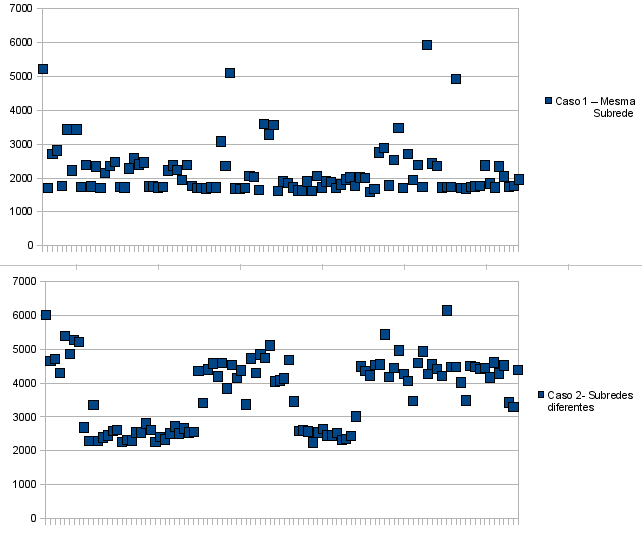
\includegraphics[width=15cm]{consulta.png} 
  \caption{Representação das medições para a consulta.}
  \label{fig:rtt}
\end{figure}

\subsection{Comparação de Desempenho entre TCP e UDP}
Para comparar os resultados de tempo de consulta entre um servidor TCP e outro UDP, vamos colocar os tempos lado a lado:

\textbf{Configuração 1: Mesma Sub-rede}
Médias do tempo de consulta:
- TCP: 1769,16 us
- UDP: 2288,52 us

Desvios padrão:
- TCP: 432,29 us
- UDP: 792,62 us

\textbf{Configuração 2: Sub-redes diferentes}
Médias do tempo de consulta:
- TCP: 9390,89 us
- UDP: 3606,54 us

Desvios padrão:
- TCP: 9758,98 us
- UDP: 1094,37 us


%\begin{figure}[htb]
%  \centering
%  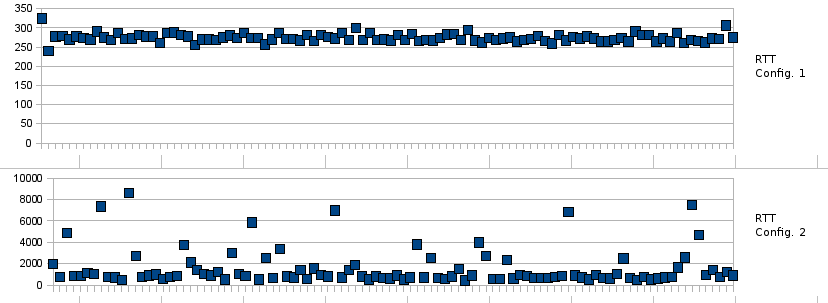
\includegraphics[width=15cm]{rtt.png} 
%  \caption{Representação das medições para o RTT.}
%  \label{fig:rtt}
%\end{figure}

Pode-se verificar a diferença considerável entre os tempos de RTT para as duas configurações. Obviamente, o tempo para abertura da conexão foi maior para a segunda 
configuração, já que os pacotes devem ser transmitidos através de roteadores e enlaces adicionais, como mostrado no resultado do traceroute acima.\\
De modo a comprovar a influência do tráfego na rede, é visível a grande diferença entre os desvios padrão em porcentagem com relação ao valor absoluto.\\


\section{Confiabilidade e Consistência}
Dois pontos a considerar: robustez quanto à comunicação e consistência dos dados.\\
Tentamos fazer todas as verificações de erros possíveis nas funções das bibliotecas de comunicação com o socket, tanto no lado cliente como no servidor. Ainda assim, não conseguimos implementar um importante caso de exceção: notificar e encerrar o cliente quando o servidor "cai".\\
Com relação à consistência dos dados, esta é garantida pela exclusão mútua nas operações de atualização de avaliação.

\section{Conclusão}
Podemos considerar que a aplicação já está totalmente funcional, todas as consultas estão funcionando corretamente, há a garantia da consistência do banco de dados do cinema e a comunicação entre cliente e servidor está boa, exceto no caso em que o servidor cai, deixando o cliente esperando por uma resposta.\\
Por utilizar o protocolo TCP, a comunicação possui todas as suas vantagens, como confiabilidade na transferência de pacotes, controle de fluxo e controle de congestionamento, o que garante uma qualidade maior à aplicação.\\
A análise de tempo também cumpriu com as espectativas, tendo uma média e um desvio padrão mais baixo para redes próximas e valores mais altos para redes mais distantes.\\
Ao fazer a aplicação em C, o nível de abstração não foi muito alto, pois tivemos que tratar muitos detalhes das conexões.\\
Podemos dizer também que fomos felizes ao utilizar um controle de conexões por threads, pois fica mais fácil de controlar do que com processos, já que quando o processo principal termina, todas as threads também terminam, evitando assim processos zumbi, além de ser mais fácil se implementar exclusão mútua de threads, por exemplo, com semáforos ou mutex lock.\\
Nosso servidor de banco de dados de cinema ainda não é um sistema completo e bem acabado, mas já provê uma base sólida para implementar aplicações gráficas e de maior porte, utilizando o servidor como o núcleo da aplicação. Pretendemos, em versões posteriores, melhorar o programa, resolver bugs e talvez, utilizar uma biblioteca gráfica para tornar sua interface mais usável. 

\section{Código Fonte}
\subsection{Makefile}
\begin{verbatim}
# Variáveis
CC = gcc
CC_FLAGS = -ggdb -Wall


# Dependências gerais
all: client server

# Cliente
client: data_access.o internet.o client.o
	$(CC) $(CC_FLAGS) data_access.o internet.o client.o -o client

client.o: client.c data_access.h internet.h defines.h
	$(CC) $(CC_FLAGS) -c client.c

# Servidor
server: data_access.o internet.o server.o
	$(CC) $(CC_FLAGS) data_access.o internet.o server.o -o server

server.o: server.c data_access.h internet.h defines.h
	$(CC) $(CC_FLAGS) -c server.c

# Bibliotecas
data_access.o: data_access.c data_access.h defines.h
	$(CC) $(CC_FLAGS) -c data_access.c

internet.o: internet.c internet.h defines.h
	$(CC) $(CC_FLAGS) -c internet.c


# Relatório (LaTeX)
relatorio:
	pdflatex relatorio.tex

# Clean
clean:
	rm *.o client server *.aux *.toc *.pdf *.log
\end{verbatim}

\subsection{repeat\_client.sh}
\begin{verbatim}
#!/bin/bash

for i in $(seq 100)
do
    ./client 143.106.150.74 < arq.in 2>> tempos.out
done
\end{verbatim}

\subsection{arq.in}
\begin{verbatim}
1
7
\end{verbatim}

\subsection{client.c}
\begin{verbatim}
//Bibliotecas comuns
#include <string.h>
#include <stdio.h>
#include <stdlib.h>
#include <netdb.h>   //Para usar o gethostbyname
#include "data_access.h"
#include "defines.h"
#include "internet.h"

//Bibliotecas para manipulacao de sockets
#include <sys/types.h>
#include <sys/socket.h>
#include <netinet/in.h>
#include <unistd.h>

//Bibliotecas para analise de tempo
#include <sys/time.h>
#include <time.h>


/* Socket único do cliente */
int socketfd;



/**************************************************************/
/******************* Funções auxiliares ***********************/

/* Função auxiliar para tratamento de entrada */
char read_option() {
  /* considera os possiveis erros e só sai quando o usuario
     digitar um caractere válido */
  
  char c, aux;
  
  while(TRUE) {
    
    /* Mensagem com as opções... */
    system("clear");
    printf("Escolha uma entre as opções e tecle Enter:\n");
    printf("(opções com (*) requererão o id do filme)\n");
    printf(" [1] Listar todas as informações de todos os filmes.\n");
    printf(" [2] Listar id e título de todos os filmes.\n");
    printf(" [3] Listar todas as informações de um filme. (*)\n");
    printf(" [4] Mostrar a sinopse de um filme. (*)\n");
    printf(" [5] Mostrar a avaliação de um filme. (*)\n");
    printf(" [6] Avaliar um filme! (*)\n");
    printf(" [7] Sair\n  ");

    c = getchar(); aux = getchar();
    if((c==SAIR || c==LISTAR_TODOS_COMPLETO || c==LISTAR_TODOS ||
				c==REG_COMPLETO || c==REG_SINOPSE || c==REG_MEDIA ||
				c==REG_AVALIAR) && aux=='\n') {
      /* se a opcao lida é válida e o próximo caractere foi Enter, 
				 retorna o caractere válido digitado*/
      return(c);
    } else {
      /* caso contrário, 'come' todo o resto da linha e volta às msgs */
      if(aux != '\n') { while(getchar()!='\n'); }
    }
  } /* fim do while */

}


/* Função auxiliar para inserção do ID no pacote 'request' */
void read_id (char *request) {

  char c;
  int dif, i = 1;

  printf(" Id: "); c = getchar();

  while (c!='\n' && i<=20) {
    request[i] = c; c = getchar(); i++;
  }

  /* right-shift de i em request[1-20] (id) */
  i --; /* i == numero de digitos */
  dif = 20 - i;
  /* caso a diferença seja 0, não precisa fazer o shift */
  if(dif != 0) {
    for (; i >= 1; i--) {
      request[i+dif] = request[i];
      request[i] = '0';
    }
  }
  return;
}


/* Função auxiliar para inserção da nota no request */
void read_nota(char *request) {
  
  char c; int i = 21;
  
  printf(" Nota (abc.de): ");
  c = getchar();
  while (c!='\n' && i<=26) {
    request[i] = c; c = getchar(); i++;
  }
  return;
}

/******************* Funções auxiliares ***********************/
/**************************************************************/





/**************************************************************/
/******[inicio] Funções que implementam os casos de uso  ******/

/* ## 1 ## */
void client_lista_todos_completo() {

  /* Recebe datagrama com número de filmes. */
  char n_filmes_str[10];
  int status, n_filmes, i;
 
  /* Espera o timeout, usando select() */
  status = client_udp_pop_buffer(socketfd, n_filmes_str, 10);
  
  /* Caso ou a pergunta ou a resposta com o n de filmes se perdeu */
  if (status == -1) {
    /* notifica usuário, envia msg de erro p/ log e retorna */
    fprintf(stderr, "ERR\n");
    printf("Request ou response perdido.\n");
    //printf("Aperte Enter para continuar..."); getchar();
    return;
  }

  n_filmes = atoi(n_filmes_str);
  if (n_filmes == 0) {
    printf("Não há filmes no servidor!\n");
    //printf("Tecle Enter para continuar..."); getchar();
    return;
  }

  printf("Número de filmes encontrados: %d\n\n", n_filmes);

  
  /* Recebe cada filme e imprime suas informações */

  char filme_str[TAM_MAX_REG]; /* 1024 */
  filme *f;
  int perdidos = 0, tam_filme;
  
  for (i = 0; i < n_filmes; i++) {

    /* recebimento do datagrama com o filme */
    status = client_udp_pop_buffer(socketfd, filme_str, TAM_MAX_REG);

    /* Caso tenha dado o timeout */
    if (status == -1) {
      /* log de erro; continua para o próximo */
      fprintf(stderr, "ERR\n");
      perdidos++; /* valor mantido para informar o usuário */
      continue;
    }
    
    /* Aloca a estrutura para guardar o filme e o seta */
    f = (filme *)malloc(sizeof(filme));
    da_str_to_filme(f, &tam_filme, filme_str);
    
    /* imprime informações completas do filme */
    da_print_full_info(f);
    printf("\n-------------------------\n");

    /* libera a memória do filme */
    da_free_all(f);
    
  }

  printf("  Filmes perdidos no transporte: %d\n\n", perdidos);
  //printf("  Tecle Enter para continuar..."); getchar();
  return;
}

/* ## 2 ## */
void client_lista_todos() {

  /* Cliente praticamente igual para a listagem completa. */
  
  char n_filmes_str[10]; int status, n_filmes, i;
 
  status = client_udp_pop_buffer(socketfd, n_filmes_str, 10);
  if (status == -1) {
    fprintf(stderr, "ERR\n");
    printf("Request ou response perdido.\n");
    printf("Aperte Enter para continuar..."); getchar();
    return;
  }

  n_filmes = atoi(n_filmes_str);
  if (n_filmes == 0) {
    printf("Não há filmes no servidor!\n");
    printf("Tecle Enter para continuar..."); getchar();
    return;
  }

  printf("Número de filmes encontrados: %d\n\n", n_filmes);

  char filme_str[TAM_MAX_REG]; /* 1024 */
  filme *f; int perdidos = 0, tam_filme;
  
  for (i = 0; i < n_filmes; i++) {
    status = client_udp_pop_buffer(socketfd, filme_str, TAM_MAX_REG);

    if (status == -1) { 
      fprintf(stderr, "ERR\n");
      perdidos++; continue;
    }
    
    f = (filme *)malloc(sizeof(filme));
    da_str_to_filme(f, &tam_filme, filme_str);
    da_print_partial_info(f); /***************************  <<-- ***/
    printf("\n-------------------------\n");
    da_free_all(f);
  }
  printf("  Filmes perdidos no transporte: %d\n\n", perdidos);
  printf("  Tecle Enter para continuar..."); getchar();
  return;
}

/* ## 3 ## */
void client_reg_completo() {

  /* leitura da resposta do servidor */
  int status;
  char filme_str[TAM_MAX_REG];
  
  status = client_udp_pop_buffer(socketfd, filme_str, TAM_MAX_REG);
  
  /* caso tenha dado timeout */
  if (status == -1) { 
    /* log erro; avisa o cliente; retorna */
    fprintf(stderr, "ERR\n");
    printf("Request ou response perdido.\n");
    printf("Aperte Enter para continuar..."); getchar();
    return;
  }
  
  /* Caso não tenha encontrado nenhum filme... */
  if (filme_str[0] == '#') {
    printf("\nFilme não encontrado.\n");
  }
  /* Caso tenha encontrado... */
  else {

    /* monta a estrutura de filme */
    filme f;
    int tam_reg;
    da_str_to_filme(&f, &tam_reg, filme_str);

    /* Imprime resultado da pesquisa */
    printf("Filme encontrado!\n\n");
    da_print_full_info(&f);
  }

  printf("\nAperte Enter para continuar..."); getchar();
  return;
}

/* ## 4 ## */
void client_reg_sinopse() {

  /* Cópia do caso de uso para a listagem completa de um filme,
     diferenciando apenas a impressão dos dados. */

  int status; char filme_str[TAM_MAX_REG];
  status = client_udp_pop_buffer(socketfd, filme_str, TAM_MAX_REG);
  
  if (status == -1) { 
    fprintf(stderr, "ERR\n");
    printf("Request ou response perdido.\n");
    printf("Aperte Enter para continuar..."); getchar();
    return;
  }
  
  if (filme_str[0] == '#') {
    printf("\nFilme não encontrado.\n");
  }
  else {
    filme f;
    int tam_reg;
    da_str_to_filme(&f, &tam_reg, filme_str);
    printf("Filme encontrado!\n\n");
    da_print_partial_info(&f); /***************************  <<-- ***/
    printf("Sinopse: %s\n", f.sinopse); /******************  <<-- ***/
  }
  printf("\nAperte Enter para continuar..."); getchar();
  return;
}

/* ## 5 ## */
void client_reg_media() {

  /* Cópia do caso de uso para a listagem completa de um filme,
     diferenciando apenas a impressão dos dados.*/

  int status; char filme_str[TAM_MAX_REG];
  status = client_udp_pop_buffer(socketfd, filme_str, TAM_MAX_REG);
  
  if (status == -1) { 
    fprintf(stderr, "ERR\n");
    printf("Request ou response perdido.\n");
    printf("Aperte Enter para continuar..."); getchar();
    return;
  }
  
  if (filme_str[0] == '#') {
    printf("\nFilme não encontrado.\n");
  }
  else {
    filme f;
    int tam_reg;
    da_str_to_filme(&f, &tam_reg, filme_str);
    printf("Filme encontrado!\n\n");
    da_print_partial_info(&f); /**********************************  <<-- */
    printf("Média: %3.2f (%d avaliações)\n", f.media, f.n_aval); /* <<-- */
  }
  printf("\nAperte Enter para continuar..."); getchar();
  return;
}

/* ## 6 ## */
void client_reg_avalia() {

  /* leitura da resposta do servidor */
  char resposta;
  int status;

  status = client_udp_pop_buffer(socketfd, &resposta, 1);

  /* caso tenha esgotado o timeout */
  if (status == -1) { 
    fprintf(stderr, "ERR\n");
    printf("Request ou response perdido.\n");
    printf("Aperte Enter para continuar..."); getchar();
    return;
  }

  /* Caso não tenha encontrado nenhum filme */
  if (resposta == '#') {
    printf("\nFilme não encontrado.\n");
  } else {
    printf("\nAvaliação realizada com sucesso!\n");
  }

  printf("\nAperte Enter para continuar..."); getchar();

  return;
}

/*******[fim] Funções que implementam os casos de uso  ********/
/**************************************************************/




int main(int argc, char** argv) {

  struct timeval tv1, tv2, tvres;
  long double total_time;
  
  /* armazena retornos de status para checagens */
  int status;

  /* Caso não haja o nome do servidor, da um erro */
  if (argc != 2) {
    fprintf(stderr, "uso: ./client <nome do servidor>\n");
    exit(1);
  }
	
  /* 
     Beej 5.8
     Remember, if you connect() a datagram socket, you can then
     simply use send() and recv() for all your transactions. 
     The socket itself is still a datagram socket and the packets
     still use UDP, but the socket interface will automatically add 
     the destination and source information for you.
  */
  /* Configura o UDP para que sempre que for enviar e receber,
     o faça para o IP e porta do servidor (bem-conhecidos). */
  socketfd = client_get_connection(argv); /* como antes */
  
  /* Nota:
     APENAS O CLIENTE estabelece essa configuração de enviar para 
     e receber de um mesmo IP/porta. Dessa forma, apenas o cliente 
     envia e recebe usando send() e recv(). Importante lembrar que 
     a comunicação continua sendo via UDP.
  */
  
  
  /* Loop da interface */
  char request[27]; /* option(1)+id(20)+nota(6) = 27  */
  memset(request, '0', 27); /* seta com os caracteres '0's */

  char c;
  c = read_option();
  request[0] = c;

  while (c != SAIR) {

    /* Conclui a montagem do pacote 'request' */
    switch(c) {
    case REG_COMPLETO:
    case REG_SINOPSE:
    case REG_MEDIA:
      read_id(request);
      break;
    case REG_AVALIAR:
      read_id(request);
      read_nota(request);
      break;
    } 

    /* Envia o pacote request ao servidor */
    status = client_udp_push_buffer(socketfd, request, 27);
    if (status == -1) {
      fprintf(stderr, "err_send\n");
      printf("UDP não conseguiu colocar a opção no buffer de \
saída. Aperte Enter e tente novamente...\n"); getchar();
    }
    /* Caso contrário, chama a função para o caso específico */
    else {
      
      switch(c) {
        case LISTAR_TODOS_COMPLETO:
          gettimeofday(&tv1, NULL); /* lê o t1 */
          client_lista_todos_completo(socketfd);
          gettimeofday(&tv2, NULL); /* lê o t2 */
          timersub(&tv2, &tv1, &tvres); /* resposta = t2 - t1 */
					/* resposta em micro-segundos */
          total_time = tvres.tv_sec*1000000 + tvres.tv_usec; 
          /* manda o tempo para a saída padrão de erro: coleta 
						 para um arquivo (via shell) */
          fprintf(stderr, "%.0Lf\n", (long double) total_time );
          break;
        case LISTAR_TODOS:
          client_lista_todos();
          break;
        case REG_COMPLETO:
          client_reg_completo();
          break;
        case REG_SINOPSE:
          client_reg_sinopse();
          break;
        case REG_MEDIA:
          client_reg_media();
          break;
        case REG_AVALIAR:
          client_reg_avalia();
          break;
      } /* [fim - switch] */
      
    } /* [fim - else] */
    
    c = read_option(); request[0] = c;
    
  }
  
  close(socketfd);
  return(0);
  
}
\end{verbatim}

\subsection{server.c}
\begin{verbatim}
// Bibliotecas comuns
#include <string.h>
#include <stdio.h>
#include <stdlib.h>
#include <netdb.h>
#include "defines.h"
#include "internet.h"
#include "data_access.h"
#include <signal.h>

// Bibliotecas para manipulacao de sockets
#include <sys/types.h>
#include <sys/socket.h>
#include <netinet/in.h>
#include <unistd.h>



/**************************************************************/
/******************* Variáveis Globais ************************/

/* Como o servidor só se comunicará por um socket, e com um 
   cliente de cada vez, essas variáveis podem ser globais, o que
   facilita sua utilização em funções auxiliares. */

/* Socket único do servidor */
int socketfd;

/* Variáveis para guardar informações do endereço do cliente */
struct sockaddr_storage client_addr;
size_t client_addr_len = sizeof(client_addr); /* necessário */

/* Variável para guardar a msg enviada pelo cliente */
char request[27];


/******************* Variáveis Globais ************************/
/**************************************************************/



/**************************************************************/
/******[inicio] Funções que implementam os casos de uso  ******/

/* ## 1 ## */
void server_lista_todos_completo() {
  
  /* Envia ao cliente:
   * -> um datagrama com número N de filmes
   * -> N datagramas: 1 para cada filme (string crua)
   */
  
  char n_filmes_str[10];
  int n_filmes, i;

  n_filmes = da_get_n_filmes();
  sprintf(n_filmes_str, "%09d", n_filmes);
  sendto(socketfd, n_filmes_str, 10, 0, (struct sockaddr *)
	 &client_addr, client_addr_len);
	
  /* Cada datagrama será montado com um vetor de caracteres de tamanho
     fixo. Esta é uma limitação necessária para o UDP */  
  char filme_str[TAM_MAX_REG];

  /* Para cada filme no arquivo... */
  for (i=1 ; i<=n_filmes ; i++) {
    
    /* seta o vetor com o i-ésimo filme no arquivo */
    da_get_raw_str(i, filme_str);

    /* envia o datagrama com o filme ao cliente */
    sendto(socketfd, filme_str, TAM_MAX_REG, 0, (struct sockaddr *)
	   &client_addr, client_addr_len);
  }
  
  return;
}

/* ## 2 ## */
void server_lista_todos() {
  /* Faz exatamente o mesmo procedimento que para a listagem 
     completa: todas as info são passadas ao cliente. */
  server_lista_todos_completo();
  return;
}

/* ## 3 ## */
void server_reg_completo() {
  
  /* leitura do id procurado */
  char id_str[21];
  int i, id;

  for (i=1; i<21; i++) { id_str[i-1] = request[i]; }
  id_str[20] = '\0'; id = atoi(id_str);
  printf("  id requisitado: %d\n", id);


  /* Realiza a busca. */
  char f_str[TAM_MAX_REG];
  int status, tam_reg;

  /* Retorna 1 se não encontrar nenhum filme. */  
  status = da_get_filme_by_id(f_str, id, &tam_reg);

  /* se não encontrou nenhum filme... */
  if (status == 1) {
    /* seta o código de erro na mensagem que irá para o cliente */
    f_str[0] = '#';
  }

  /* envia o filme (ou código de erro) ao cliente */
  sendto(socketfd, f_str, TAM_MAX_REG, 0, (struct sockaddr *)
	 &client_addr, client_addr_len);

  return;
}

/* ## 4 ## */
void server_reg_sinopse() {
  /* Neste caso, o servidor faz exatamente o mesmo
   * que na listagem completa de um registro:
   * 1- Recebe o registro procurado;
   * 2- Faz a busca;
   * 3- Se não encontrar o filme, retorna o caractere '#'
   * 4- Se encontrar, retorna a string crua do filme
   */
  server_reg_completo();
  return;
}

/* ## 5 ## */
void server_reg_media() {
  /* Neste caso, o servidor faz exatamente o mesmo
   * que na listagem completa de um registro:
   * 1- Recebe o registro procurado;
   * 2- Faz a busca;
   * 3- Se não encontrar o filme, retorna o caractere '#'
   * 4- Se encontrar, retorna a string crua do filme
   */
  server_reg_completo();
  return;
}

/* ## 6 ## */
void server_reg_avalia() {

  /* leitura do id procurado */
  char id_str[21];
  int i, id;

  for (i=1; i<21; i++) { id_str[i-1] = request[i]; }
  id_str[20] = '\0'; id = atoi(id_str);
  printf("  id requisitado: %d\n", id);

  /* leitura da nota */
  char nota_str[7];
  float nota;
  for (i=21; i<=26; i++) { nota_str[i-21] = request[i]; }
  nota_str[6] = '\0'; nota = atof(nota_str);
  printf("  nota enviada: %06.2f", nota);

  /*
   * Função que realiza a avaliação:
   * Retorna 1 se o filme não existe.
   * Retorna 0 se ocorreu tudo bem.
   */
  /* Nota: Esta função não requer mais exclusão mútua, pois o 
     servidor agora é iterativo e só um processo/thread pode
     querer escrever no arquivo por vez. */
  int status;
  status = da_avalia_filme(id, nota); 

  /* 
   * Prepara o caractere de resposta:
   * Caso o filme não exista, responde '#'
   * Caso contrário, confirma a avaliação com '%'
   */
  char resposta;
  if (status == 1) { resposta = '#'; }
  else { resposta = '%'; }

  /* envia um datagrama com apenas um caractere, o de resposta */
  sendto(socketfd, &resposta, 1, 0, (struct sockaddr *)
	 &client_addr, client_addr_len);
  
  return;
}

/*******[fim] Funções que implementam os casos de uso  ********/
/**************************************************************/





/* Trata o sinal de interrupção */
void trata_SIGINT(int sig) {
  printf("\nEncerrando o servidor...\n");
  close(socketfd);
  exit(0);
}



int main() {
  
  signal(SIGINT,trata_SIGINT);
  
  int status;
  struct addrinfo opcoes;
  struct addrinfo *servinfo; // Informações do meu endereço
  
  memset(&opcoes, 0, sizeof(opcoes)); // zera a estrutura
  opcoes.ai_family = AF_INET;         // IPv4
  opcoes.ai_socktype = SOCK_DGRAM;    // UDP datagram sockets
  opcoes.ai_flags = AI_PASSIVE;       // fill in my IP for me

  status = getaddrinfo(NULL, SERVER_PORT_STR, &opcoes, &servinfo);
  if (status != 0) {
    fprintf(stderr, "getaddrinfo error: %s\n", gai_strerror(status));
    exit(1);
  }

  /* Cria o socket e o associa a uma porta */
  socketfd = socket(servinfo->ai_family, servinfo->ai_socktype, 
		    servinfo->ai_protocol);
 
  status = bind(socketfd, servinfo->ai_addr, servinfo->ai_addrlen);
  if (status == -1) {
    fprintf(stderr, "error on binding the socket to a port\n");
    exit(1);
  }
  freeaddrinfo(servinfo);
  printf("Socket UDP criado!\n");
  

  /* Loop infinito de recebimento e tratamento das mensagens */
  while (TRUE) {
    printf("Aguardando request...\n");

    /* Esta função bloqueia o servidor até que chegue um pacote. 
       O endereço do cliente é setado! */
    status = recvfrom(socketfd, request, 27, 0, (struct sockaddr *)
		      &client_addr, (socklen_t *) &client_addr_len);

    printf("Opção recebida: %c\n", request[0]);
    
    /* "O que vc quer, cliente?!" */
    switch(request[0]) {
      
    case LISTAR_TODOS_COMPLETO:
      server_lista_todos_completo();
      break;
    case LISTAR_TODOS:
      server_lista_todos();
      break;
    case REG_COMPLETO:
      server_reg_completo();
      break;
    case REG_SINOPSE:
      server_reg_sinopse();
      break;
    case REG_MEDIA:
      server_reg_media();
      break;
    case REG_AVALIAR:
      server_reg_avalia();
      break;
    }

    /* volta ao início do loop principal */

  }


  /* Processo servidor executa em loop infinito */
}
\end{verbatim}

\subsection{defines.h}
\begin{verbatim}
#define TRUE 1
#define FALSE 0

#define LISTAR_TODOS_COMPLETO '1'
#define LISTAR_TODOS '2'
#define REG_COMPLETO '3'
#define REG_SINOPSE '4'
#define REG_MEDIA '5'
#define REG_AVALIAR '6'
#define SAIR '7'


// A Porta em que o servidor escuta
#define SERVER_PORT 50000
#define SERVER_PORT_STR "50000"

// Tempo limite de espera por resposta do servidor, em MICRO seg
#define TIMEOUT 50000 /* 50000us = 50ms */

// Estrutura para definir o atributo a ser passado para a thread
typedef struct {
  int connect_socket;
  int thr_index;
} thread_attr ;
\end{verbatim}

\subsection{internet.h}
\begin{verbatim}
/* Funções para auxiliar nas operações com os sockets  */

/* Retorna o socketfd da "conexão" com o servidor */
/* Note que como estamos usando datagram_socket (UDP),
   essa conexão funciona apenas como uma configuração. */
int client_get_connection(char **argv);

/* Envia um buffer por datagrama (UDP) */
int client_udp_push_buffer (int socket, char *buffer, int n);

/* Recebe o datagrama enviado pelo servidor. 
   Implementa o time-out com o uso do select() 
   Retorna -1 caso tenha esgotado o timeout. */
int client_udp_pop_buffer (int socket, char *buffer, int n);
\end{verbatim}

\subsection{internet.c}
\begin{verbatim}
//Bibliotecas comuns
#include "internet.h"
#include "defines.h"
#include "data_access.h"
#include <string.h>
#include <stdio.h>
#include <stdlib.h>
#include <netdb.h>

//Bibliotecas para manipulacao de sockets
#include <sys/types.h>
#include <sys/socket.h>
#include <netinet/in.h>
#include <unistd.h>

//Bibliotecas para analise de tempo
#include <sys/time.h>
#include <time.h>


/* Retorna o socketfd da "conexão" com o servidor */
/* Note que como estamos usando datagram_socket (UDP),
   essa conexão funciona apenas como uma configuração. */
int client_get_connection(char **argv) {

  int status, socketfd;
  struct addrinfo opcoes;
  struct addrinfo *servinfo;  // will point to the results

  memset(&opcoes, 0, sizeof(opcoes)); // zera a estrutura
  opcoes.ai_family = AF_INET;         // IPv4
  opcoes.ai_socktype = SOCK_DGRAM;    // UDP datagram sockets
  opcoes.ai_flags = AI_PASSIVE;       // fill in my IP for me

  status = getaddrinfo(argv[1], SERVER_PORT_STR, &opcoes, &servinfo);
  if (status != 0) {
    fprintf(stderr, "getaddrinfo error: %s\n", 
	    gai_strerror(status));
    exit(1);
  }
  
  /* cria o socket com os parâmetros setados */
  socketfd = socket(servinfo->ai_family, servinfo->ai_socktype, 
		    servinfo->ai_protocol);

  /* faz a conexão com o socket do servidor */
  status = connect(socketfd, servinfo->ai_addr, servinfo->ai_addrlen);
  
  /* Caso dê algum erro na conexão, pára o cliente */
  if (status == -1){
    fprintf(stderr, "Problema na conexão.\n");
    exit(1);
  }
  
  /* libera a estrutura de informações do servidor */
  freeaddrinfo(servinfo);
  return(socketfd);
  
}


/* Envia um buffer por datagrama (UDP) */
int client_udp_push_buffer (int socket, char *buffer, int n) {
  
  /*
    Entradas:
    n - número de caracteres a serem escritos;
    buffer - buffer de onde se lê.
  */
  
  int i = 0;
  while (i == 0) {
    i = send(socket, buffer, n, 0);
  }
  return(i);
}


/* Recebe o datagrama enviado pelo servidor. 
   Implementa o time-out com o uso do select() 
   Retorna -1 caso tenha esgotado o timeout. */
int client_udp_pop_buffer (int socket, char *buffer, int n) {
  
  struct timeval timeout; 
  fd_set read_fd_set; /* conjunto de fd's de leitura */

  /* seta o valor para o timeout */
  timeout.tv_sec = 0; 
  timeout.tv_usec = TIMEOUT;

  /* limpa o conjunto de fd's e adiciona o socket */
  FD_ZERO(&read_fd_set);
  FD_SET(socket, &read_fd_set); 

  /* bloqueia até que o socket esteja pronto ou
     acabe o timeout */
  select(socket+1, &read_fd_set, NULL, NULL, &timeout);

  /* Caso tenha chegado alguma mensagem, retorna o n de 
     bytes lidos */
  if (FD_ISSET(socket, &read_fd_set)) {
    return(recv(socket, buffer, n, 0));
  }
  /* Caso esgote o tempo, retorna -1 */
  else {
    return(-1);
  }
  
}
\end{verbatim}

\subsection{data\_access.h}
\begin{verbatim}
#define TAM_MAX_REG 1024 /* 1kB */
#define TAM_MAX_TIT 30
#define TAM_MAX_SIN 900
#define TAM_MAX_SALA 20
#define TAM_MAX_HOR 20

#define TAM_MAX_ATR 900

/* n max de digitos do tamanho do registro e do id */
#define TAM_REG_ID 20 

/* abc.de (valor de 0 a 100, com 2 dígitos decimais) */
#define TAM_MEDIA 6 

/* cada filme pode ter até 9999 avaliações */
#define TAM_N_AVALIACOES 4 

typedef struct {
  int id;
  char *titulo;
  char *sinopse;
  char *sala;
  char *horarios;
  
  int n_aval; /* número de avaliações */
  float media;
  
  struct filme *prox_filme;
} filme;


/**** Funções a serem chamadas externamente (API) *****/
/*            'da' refere-se a data access            */


/* Retorna o i-ésimo filme do arquivo */
void da_get_raw_str (int index, char *f_str);

/* Faz um parse da string lida do arquivo para um filme */
int da_str_to_filme(filme *f_ret, int *tam_reg, char *f_str);

/* Libera as strings alocadas dinamicamente */
void da_free_strs(filme *f);

/* Imprime as informações já formatadas de um filme */
void da_print_full_info(filme *f);

/* Imprime as informações já formatadas de um filme */
void da_print_partial_info(filme *f);

/* Função que retorna um filme a partir de um id */
int da_get_filme_by_id(char *f_str, int id, int *tamanho);

/* Libera toda a memória alocada para o(s) filme(s) (strings 
   e struct) e retorna o numero de filmes desalocados */
int da_free_all(filme *f);

/* Retorna o número de filmes no arquivo */
int da_get_n_filmes();

/* Atualiza o arquivo com a nova avaliação */
int da_avalia_filme(int id, float nota);

\end{verbatim}

\subsection{data\_access.c}
\begin{verbatim}
#include <stdio.h>
#include <stdlib.h>
#include "data_access.h"

/* Retorna o i-ésimo filme do arquivo */
void da_get_raw_str (int index, char *f_str) {
  
  FILE *arq;
  int tam_reg, i = 0;
  long int cursor = 0; /* indice de leitura do arquivo */

  arq = fopen("filmes.dat", "r");

  /* Enquanto houver registros no arquivo */
  while(fscanf(arq, "%d@", &tam_reg) != EOF) {
    i++;
    fseek(arq, cursor, SEEK_SET); /* pula p/ o inicio do registro */

    /* caso seja o filme procurado, seta a string de retorno */
    if (i == index) {
      fgets(f_str, tam_reg, arq);
      break;
    }

    /* ajuste para a leitura do próximo reg no arq */
    cursor += tam_reg; 
  }
  
  fclose(arq);
  
  return;
}

/* Faz um parse da string lida do arquivo para um filme */
int da_str_to_filme (filme *f_ret, int *tam_reg, char *f_str) {
  /* Entrada: string crua de um filme lida do arquivo */
  /* Saída:
     - setup da struct filme passada por referência 
     - tamanho do registro no arquivo
     - valor numérico para erros */

  /* Formato do registro no arquivo */
  /* Como há atributos de texto, é difícil manter os registros 
     com tamanho constante no arq. Assim, uma ideia é usar 
     separadores entre os atributos */

  /* [tam][id][aval][media][tit][sinopse][sala][horarios]
     int tam_total_do_reg (incluindo todos os separadores), 
     int id, int avaliacoes, float media [TAMANHO FIXO NO ARQUIVO!], 
     string titulo, string sinopse, string sala, string horarios.
     Separador: @
  */

  char str[TAM_MAX_ATR]; /* comporta qq atributo */

  int i = 0; /* índice de acesso de f_str */
  int j = 0; /* indice para montagem da string  */

  /* tamanho do registro */
  while(f_str[i]!='@') {
    str[j] = f_str[i];
    i++; j++;
  }
  str[j] = '\0';
  *tam_reg = atoi(str);

  /* id */
  i++; j = 0;
  while(f_str[i]!='@') { str[j] = f_str[i]; i++; j++; }
  str[j] = '\0'; 
  f_ret->id = atoi(str);

  /* numero de avaliações */
  i++; j = 0;
  while(f_str[i]!='@') { str[j] = f_str[i]; i++; j++; }
  str[j] = '\0';
  f_ret->n_aval = atoi(str);
	
  /* média */
  i++; j = 0;
  while(f_str[i]!='@') { str[j] = f_str[i]; i++; j++; }
  str[j] = '\0';
  f_ret->media = atof(str);
	
  /* titulo */
  i++; j = 0;
  while(f_str[i]!='@') {
    str[j] = f_str[i];
    i++; j++;
  }
  str[j] = '\0';
  /* aloca a string dinamicamente */
  f_ret->titulo = (char *)malloc((j+1)*sizeof(char));
  sprintf(f_ret->titulo, "%s", str);

  /* Blocos de código similares ao de cima, comprimidos */
  /* sinopse */
  i++; j = 0;
  while(f_str[i]!='@') { str[j] = f_str[i]; i++; j++; } 
  str[j] = '\0'; 
  f_ret->sinopse = (char *)malloc((j+1)*sizeof(char));
  sprintf(f_ret->sinopse, "%s", str);

  /* sala */
  i++; j = 0;
  while(f_str[i]!='@') { str[j] = f_str[i]; i++; j++; }
  str[j] = '\0';
  f_ret->sala = (char *) malloc((j+1)*sizeof(char));
  sprintf(f_ret->sala, "%s", str);

  /* horarios */
  i++; j = 0;
  while(f_str[i]!='@' && f_str[i]!='\0') { 
    str[j] = f_str[i]; i++; j++; 
  } 
  str[j] = '\0';
  f_ret->horarios = (char *) malloc((j+1)*sizeof(char));
  sprintf(f_ret->horarios, "%s", str);

  /* next - lembra dele? :) */
  f_ret->prox_filme = NULL;

  return(0);
}


/* Imprime as informações já formatadas de um filme */
void da_print_full_info(filme *f) {
  printf("Id: %d\n", f->id);
  printf("Titulo: %s\n", f->titulo);
  printf("Sinopse: %s\n", f->sinopse);
  printf("Sala: %s\n", f->sala);
  printf("Horários: %s\n", f->horarios);
  printf("Média: %06.2f (%d avaliações)\n", 
	 f->media, f->n_aval);
  return;
}

/* Imprime as informações já formatadas de um filme */
void da_print_partial_info(filme *f) {
  printf("Id: %d\n", f->id);
  printf("Titulo: %s\n", f->titulo);
  return;
}


/* Libera as strings alocadas dinamicamente */
void da_free_strs(filme *f) {
  free(f->titulo);
  free(f->sinopse);
  free(f->sala);
  free(f->horarios);
  return;
}


int da_free_all(filme *f) {
  /* Esta função desaloca todos os filmes que estiverem na 
     lista, e retorna o número desses filmes que foram desa-
     locados. A lista precisa ser resolvida de trás pra 
     frente, por isso está sendo usada recursão. */

  int i;

  da_free_strs(f);

  /* Condição de parada (último filme) */
  if(f->prox_filme == NULL) {
    free(f);
    return(0); /* retorna, inicializando contador */
  }

  /* Chamada recursiva */
  /* cast pro -Wall n reclamar */
  i = da_free_all((filme *)f->prox_filme);

  /* Resolvida a recursão, libera a struct e retorna */
  free(f);
  return(i);
}
	

/* Função que retorna um filme a partir de um id */
int da_get_filme_by_id(char *f_str, int id, int *tamanho) {

  /* Função responsável por acessar o arquivo dos registros,
     buscar o filme com o id igual ao passado como argumento,
     e retornar o resultado da busca
     Saídas: 0 - filme encontrado (setado em f_str)
     1 - código de retorno que indica que nada foi encontrado
  */

  int tam_reg, id_reg;
  long int cursor = 0; /* indice de leitura do arquivo */
  FILE *arq;

  arq = fopen("filmes.dat", "r");

  while(fscanf(arq, "%d@%d@", &tam_reg, &id_reg) != EOF) {
    /* registro encontrado */
    if(id_reg == id) {
      /* caminha no arquivo até o inicio do registro */
      fseek(arq, cursor, SEEK_SET);
      fgets(f_str, tam_reg, arq);
      *tamanho = tam_reg;
      fclose(arq);
      return(0);
    } else {
      cursor += tam_reg;
      fseek(arq, cursor, SEEK_SET);
    }
  } /* só vai sair do while se não encontrar o filme */
  
  fclose(arq);
  
  return(1);

}


/* Retorna o número de filmes no arquivo */
int da_get_n_filmes() {

  FILE *arq;
  int tam_reg, i = 0;
  long int cursor = 0; /* indice de leitura do arquivo */

  arq = fopen("filmes.dat", "r");

  /* Enquanto houver registros no arquivo */
  while(fscanf(arq, "%d@", &tam_reg) != EOF) {
    i++;
    /* pula p/ o inicio do registro */
    fseek(arq, cursor, SEEK_SET); 

    /* ajuste para a leitura do próximo reg no arq */
    cursor += tam_reg; 
  }
  
  fclose(arq);
  
  return(i-1);
	
}

/* Atualiza o arquivo com a nova avaliação */
int da_avalia_filme(int id, float nota) {
  /* Retorno
     1 - O filme com o id passado não existe
     0 - Atualização efetuada.
  */

  int tam_reg, id_reg, n_aval;
  float media;
  long int cursor = 0; /* indice de leitura do arquivo */
  FILE *arq;

  /* abre o arquivo com permissão para escrita */
  arq = fopen("filmes.dat", "r+");

  while(fscanf(arq, "%d@%d@%d@%f@", &tam_reg, &id_reg, 
	       &n_aval, &media) != EOF) {
    /* registro encontrado */
    if(id_reg == id) {
      /* Cálculo da nova média para o filme */
      float nova_media;
      nova_media = (media*n_aval + nota)/(n_aval+1);
      
      /* caminha no arquivo até o início do n de avaliações */
      fseek(arq, -(2/*@s*/ + TAM_MEDIA + TAM_N_AVALIACOES), 
	    SEEK_CUR);

      /* Atualização dos valores: n de avaliações e média */
      fprintf(arq, "%04d@%06.2f@", n_aval+1, nova_media);

      fclose(arq);
      return(0);
    } else {
      cursor += tam_reg;
      fseek(arq, cursor, SEEK_SET);
    }
  } /* só vai sair do while se não encontrar o filme */
  
  fclose(arq);
  
  return(1);

}
\end{verbatim}



%\section{Anexo}
%\begin{figure}[htb]
%  \centering
%  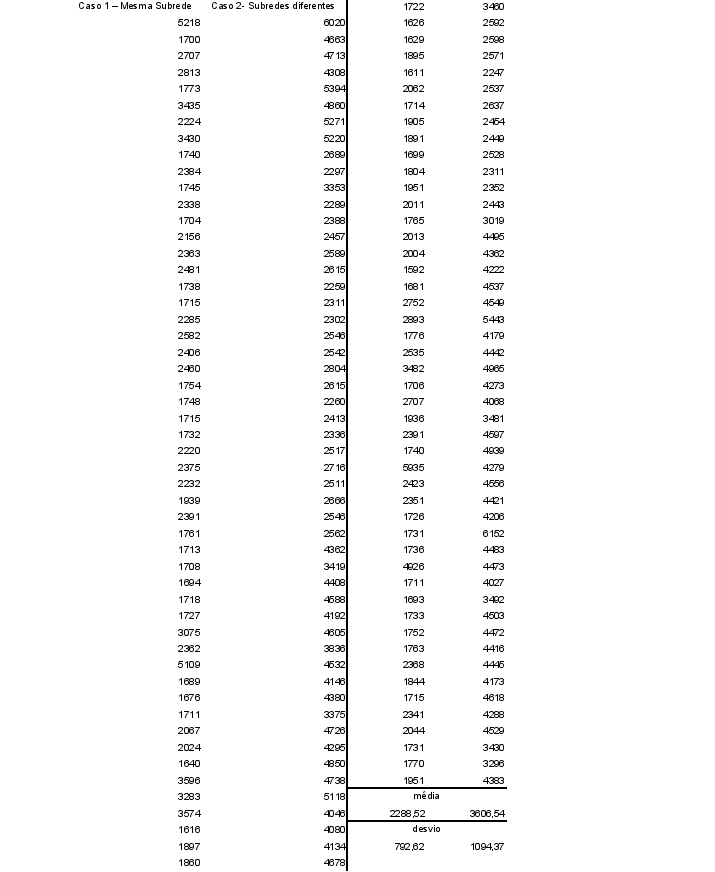
\includegraphics[width=15cm]{medicoes.png} 
%  \caption{Representação das medições para a consulta.}
%  \label{fig:rtt}
%\end{figure}

\begin{thebibliography}{99}
\bibitem{R1} HALL, Brian. Beej's Guide to Network Programming. Disponível em: http://http://beej.us/guide/bgnet/output/html/multipage/index.html.
\end{thebibliography}

\end{document}
